\documentclass[12pt,a4paper]{scrartcl}
\usepackage[utf8]{inputenc}
\usepackage[english]{babel}
\usepackage{amsmath}
\usepackage{amsfonts}
\usepackage{amssymb}
\usepackage[T1]{fontenc}
\usepackage{ae,aecompl}
\usepackage{graphicx}
\usepackage{wrapfig} 
%\usepackage{subfig} % see here: https://tex.stackexchange.com/questions/13625/subcaption-vs-subfig-best-package-for-referencing-a-subfigure
\usepackage{subcaption} % support subplots
\usepackage{caption}
\usepackage{pdfpages}
\usepackage{geometry}
 \geometry{
 a4paper,
 total={160mm,240mm},
 left=25mm,
 top=30mm,
 }
\usepackage{times}
\parindent0pt 

\graphicspath{ {_illustrations/} }

  \usepackage[%
%    %%% general options
%    pdftex=true,      %% sets up hyperref for use with the pdftex program
%    %plainpages=false, %% set it to false, if pdflatex complains: ``destination with same identifier already exists''
%    %
%    %%% extension options
%    backref,      %% adds a backlink text to the end of each item in the bibliography
%    pagebackref=false, %% if true, creates backward references as a list of page numbers in the bibliography
	hidelinks,
    colorlinks=false,   %% turn on colored links (true is better for on-screen reading, false is better for printout versions)
%    linkcolor=blue,
%    citecolor=blue,    
%    %%% PDF-specific display options
    bookmarks=true,          %% if true, generate PDF bookmarks (requires two passes of pdflatex)
    bookmarksopen=true     %% if true, show all PDF bookmarks expanded
%    bookmarksnumbered=false, %% if true, add the section numbers to the bookmarks
%    %pdfstartpage={1},        %% determines, on which page the PDF file is opened
%    pdfpagemode=None         %% None, UseOutlines (=show bookmarks), UseThumbs (show thumbnails), FullScreen
  ]{hyperref}


%%% title
\title{Satellite Data Labeling with QGIS}
\subtitle{A Guide to Digitizing Roads}
%%% author(s)
\author{Erik Seiert (minor additions by Harald Hentschke)}

%%% date
\date{Tübingen, \today{}}

\begin{document}


\maketitle
\newpage

\newpage
\tableofcontents
\newpage
 
\section{A short introduction to QGIS}

Changes by Harald:

\begin{itemize}
	\item updated shell code to obtain most current key for QGIS (from 2019, as of Aug 08 2019)
	\item made all links clickable
	\item amended section on installation: /etc/apt/sources.list
	\item added general guidelines on the quality of labeling and accompanying exemplary images
\end{itemize}

\textbf{Whats QGIS?} 


QGIS is a Geographic Information System (Software) $\rightarrow$ GIS. 
It is free and open source, which means, it is available for anyone at no cost.  \newline

QGIS bundles many tools in one program to allow the complete workflow from initial data visualisation over 
complex analysis to complete maps ready for the use by officials, scientists, hikers or you.  

In this document we will cover some general basics and then focus on the workflow of labelling 
satellite data. \newline

\subsection{Installing QGIS}

I generally recommend to download the Long Term Release (LTR, currently QGIS 3.4.8) of QGIS to avoid any issues. \newline

\textbf{Linux: Installation for Debian/Ubuntu, also tested with Linux Mint 19} \newline
\textit{resource: \url{https://qgis.org/en/site/forusers/alldownloads.html\#debian-ubuntu}} \newline 

I assume you have at least rudimentary knowledge of terminal use in Linux. \newline
Otherwise read this: 
\url{https://www.linode.com/docs/tools-reference/tools/using-the-terminal/} \newline
or this: 
\url{https://www.howtogeek.com/140679/beginner-geek-how-to-start-using-the-linux-terminal/} \newline

First, add the QGIS repository to get the newest stable version of QGIS.
This requires to add the qgis.org repository public key to your apt keyring, type:

\begin{verbatim}
wget -O - https://qgis.org/downloads/qgis-2019.gpg.key | gpg --import
gpg --fingerprint 51F523511C7028C3
\end{verbatim}

You can verify the key on this page: \url{https://qgis.org/en/site/forusers/alldownloads.html\#debian-ubuntu}
Now you need to add the key to apt:  

\begin{verbatim}
gpg --export --armor 51F523511C7028C3 | sudo apt-key add -
\end{verbatim}

Next, you have to add specific lines to your /etc/apt/sources.list file.
Be sure to change the version number to your version of Ubuntu or Debian. \newline
This is an example of the entries for the long term release of qgis on Ubuntu 18.04 bionic:

\begin{verbatim}
deb     https://qgis.org/ubuntu-ltr bionic main
deb-src https://qgis.org/ubuntu-ltr bionic main
\end{verbatim}


With the key added to your apt keyring and the repository added to the sources.list file, you can install QGIS:  

\begin{verbatim}
sudo apt-get update
sudo apt-get install qgis python3-qgis qgis-plugin-grass
\end{verbatim}

With these steps you should be set up and ready to start with chapter \ref{step2}. \newline

\textbf{MacOS} \newline

To install on MacOS, download the long term release on:
\url{https://qgis.org/en/site/forusers/download.html} and follow the steps described in the installer. Done.\newline

\textbf{Windows} \newline

I recommend using the OSGeo4W network installation method. \newline
The installer can be found here: \url{https://qgis.org/en/site/forusers/download.html} (Download for windows).

OSGeo4W is a package manager allowing you to install the most recent stable versions of QGIS
I will describe the installation process for you here: \newline

\begin{itemize}

\item When downloaded, open the installer
\item Select advanced install
\item Select install from the internet
\item choose a root directory 
\item leave the package directory at default
\item use direct connection if not specified otherwise
\item (next)
\item Now there should be a list of Package Repositories
\item click the "+" next to Desktop
\item find the package with name "qgis-ltr"
\item click on the arrow symbol to the left of the row
\item now it should show a version like 3.4.10 or something

\item OPTIONAL: 
\item you can select GRASS GIS and SAGA in the same way (needed for some tools in QGIS)

\end{itemize}

By clicking "next", some dependencies will pop up (just click next and dont change anything in this window).
The dependencies will be downloaded and installed along with qgis.\newline

You are ready to start.

\subsection{Basic project set up}
\label{step2}

I assume you already have downloaded the data youre planning to work with.
Now, be sure to place the data in a well ordered folder structure, this will qgis
make life a lot easier. \newline

Suggested Paths, please create the folders in the way described below:

\begin{verbatim}
{path to your datafolder} / Labelling Project / Satellite Images
{path to your datafolder} / Labelling Project / Labels
\end{verbatim}


{\large \textbf{Start QGIS}} \newline
Once qgis is started, you can set up a project in which the data labelling will take place. 
Open the project properties either by pressing \textit{ctrl + shift + p} or click \textit{Project} and then \textit{Properties}.\\

A window will pop up displaying the general settings. \\
Set the project path to \textit{ (path to your datafolder) / Labelling Project}

Optionally you can set a project title.
Be sure that the "Save Paths" option is \textit{relative}.\\

\textbf{The Measurements Rider}  \\
By default, the calculations ellipsoid should be set to "WGS 84". 
Leave the default, as it is a widely used reference.
Change only if you know what you are doing/ there are problems with display of certain layers. \\
All other options in this rider should be in the metric system to avoid complications.\\

\textbf{The Coordinate Display Rider} \\
I recommend to change the option "display coordinates" to decimal degrees which is the same as the google maps 
display style.

\subsubsection{Coordinates: datum and system}

Change to the Menu Item "CRS".
Here you can check if the Project Coordinate Reference System is also set to WGS 84. 
If not, you can change it by Filtering/Searching for 4326 which is the EPSG number of the WGS 84 system.  \\

For reference purposes, you can set the Coordinate System to WGS84/ Pseudo Mercator (EPSG: 3857).  
This coordinate system is used by google maps, which you may want to use to double-check locations.

\subsubsection{Useful windows and features}

By default QGIS displays a few windows with useful features.
I recommend to place the "Browser" Window at the right side of the screen, this window should show your project 
folder as "Project Home"  and all the sub-folders and files.

If the "Processing Toolbox" window is not displayed (something you may need soon): \\
Click on "View" - "Panels" - "Processing Toolbox" \\

\textbf{Hint:} In this menu you can turn on and off any panels you like.

\subsection{Plugins}

Plugins are a nice way to extend the functionality of QGIS.

Navigate to the Plugins Menu: \\
Click on "Manage and Install Plugins" (depending on you internet connection this may take a while to open). \\
In the plugin manager you have the possibility to install plugins from a QGIS plugin repository. \\
Here you can easily search for both, installed and available plugins in the repository, the settings can be left at default for now.

\subsubsection{The Semi-Automatic Classification Plugin (SCP)}

A Plugin we will frequently use is the SCP. Search for the "SCP" plugin in the search field of the plugin manager.
Click install and wait, downloading and installing may take a while.

\subsubsection{The coordinate capture plugin}
\label{coordcap}

This is a useful little tool to quickly extract coordinates from a map canvas. \\
In the vectors menu, next right to the plugins menu, click on \textit{coordinate capture}. \\
A window will show up (probably docked on the left side of the main window). \\
From there you can click \textit{start capture} and get the coordinates of a clicked point on the screen

\subsection{Data: Their types, and how to load them}

Here i will give a short introduction to the data types most common to any GIS

\subsubsection{Raster data}
\label{rastabands}

Raster Data are discrete, rectangular data matrices.
Each cell of the "Matrix" has a single value and is situated (without any no-data space in between) next to other cells (exept where the borders of the images are of course). \\
Each cell of the raster is also defined by coordinates and a width in X,Y direction (which is the resolution).
An example for raster data are the satellite images you will be labelling. \\

The cell value can be a height, a brightness (0-255) or a color value (either one of red, green and blue).
Rasters of red, green and blue values are combined into RGB images, displaying a color image.  
Cells of the same raster never overlap. \\

\textbf{Excurse: Raster Bands} \newline
Get the semiautomatic classification manual for information about which band contains which wavelength data for 
some of the most widespread satellite platforms: 
\url{https://fromgistors.blogspot.com/p/user-manual.html}\\

You dont need to read the full manual. 
It pays though to have a look at the chapter \textit{Brief introduction to remote sensing}.
There are tables for the image bands of the most common satellite platforms with their ordering of wavelengths/ their names and resolutions.

There is also the combined imagery product specification from planet.com available at: \\
\url{https://www.planet.com/products/planet-imagery/} \\
Scroll down to the button "Download full specs". \\
You are most likely using the Analytic Ortho Scene Product or any other analytic scene.
planet.com did not list their bands according to numbers in the attribute table, i guess the the word order of the band listing seems sufficient to them.
Be sure to check which product you have: 3 or 4 band images (4 band would be better).  
\textit{(Excurse end)}. \\

\textbf{Common file type:} \\

The .tif or .tiff or any .gtiff variation is very common to save raster data, you will most likely work with these file types when you do the labelling job.  

Tiff files can contain multiple bands/ layers of images such as but not limited to the RGB layers of a satellite image,
where each band would correlate to a different sensor of the satellite.
Different satellite platforms have different ways of saving their data: 
The landsat 8 for example does save each of their bands in a separate file while planet.coms ortho analytic scene comes already combined. 

\subsubsection{Vector data}

The most basic Vector Data are Points. The most Basic Attribute vector data can have are coordinates. 
Vector data can have any number of attributes (e.g. temperature, time, concentration, precipitation, average number of people etc. etc. etc.). \\

Next step from points are lines and multi-point lines.
As the smart reader will already have concluded, lines are made of 2 points at least.
We will be creating a lot of line features during the labelling of the satellite images.\\

Another step further down the complexity line are polygons. 
They are made up of a closed multipoint line and generally have a colored filling.
This filling shows an area with an attribute of the same value. \\

\textbf{Common Filetypes:}\\

The esri shape file: .shp. \\
This is a common vector data format, which actually composes of MULTIPLE different files with the same name but different file endings.
If you save vector data to the .shp format you will usually get six files of the same name and different file endings.
When sending these data, it is IMPORTANT to send all the files along with the .shp file. 
Otherwise we will not be able to use the data.\\

google .kml or .kmz files \\
These data formats are quite easy to handle as they are just single files containing all the necessary information.

\section{Loading the data}
\label{step3}

Now, that we know a bit about the data types we are going to handle, we can start loading the data. \\
There are multiple ways to do that:  

\begin{enumerate}
\item Drag and Drop from the project folder into the main window (works over QGIS' browser window)

\item Click \textit{Layer} - \textit{Add Layer} - \textit{Add Raster Layer} - click the \textit{...} button
\begin{enumerate}
\item Choose the satellite image from your Sat Image folder and click \textit{open}
\end{enumerate}

\end{enumerate}

The display of the data can be managed in the layer window (optimally at the left side of the screen). 
There you can change the order of display by drag'n drop and disable/enable the layers by unchecking the checkbox. 
% open properties/ additional information by right clicking

\textbf{Hint:} Useful feature: \textit{Zoom to Layer} which allows you to quickly display layers on the screen in full size.  

\subsection{Preparing the data with the SCP plugin}
\label{scpprep}

Now that the data are loaded, it is time to prepare them for further processing.  
After you have loaded the Image/ Image bands into QGIS, open the SCP window (should be a green/ yellow sign with a white "+" inside) on the very left of the toolbar. \\

The menu point Band Set should be selected, if not do so now. 
Here you can choose your rasters: either multiband or single band and define them in the band set below.
This happens automatically when a multiband tif is loaded. \\

Now we need some information from meta data files of our images to complete our \textit{band set definition}.
For planet.com images, there should be an .xml file, which can be opened by any text editor.  
There, at the end of the file should be multiple categories: \textit{bandSpecificMetadata}.  
From the SubCategory \textit{ps:reflectanceCoefficient} you can copy the Multiplicative Factor for each band. \\

The center wavelength can be found in the documentation of the planet.com products. 
(Chapter: \textit{2.1 PLANETSCOPE SATELLITE CONSTELLATION AND SENSOR CHARACTERISTICS})
You need to calculate the arithmetic mean for each of the bands, as there are only minimum and maximum value given. \\

For Landsat Data, there are automatic steps. The pre-processing is described in the SCP manual. \\

Now, click on the \textit{Basic tools} menu point of the SCP window.
The rider \textit{RGB list} should be open. There, click the button next to "Band Combinations" (Bottom of the window). Click yes and close the window.

\section{The labeling}

Before we begin with the actual labelling, we have to take a few additional steps:
One will be necessary to actually make the labels you created usable for others. \\
The other will make your labeling live a lot easier. 

\subsection{Vector layer creation}

Of course we first need to create a layer to fill it with data. This is done in the following way:  

\begin{itemize}
\item Click on the \textit{Layer} Menu Item - \textit{Create Layer} - \textit{New Shape File Layer}
\item Choose an appropriate, identifiable filename (such as YYYY\_MM\_DD\_REGION\_roadlabels.shp) 
\item keep the file encoding at UTF8! Change it to UTF8 if it is not.
\item change the geometry type to \textbf{line}
\item be sure to keep the coordinate system at WGS 84 if not specified otherwise
\item click ok
\end{itemize}

\subsection{Get an overview \newline band combinations}

It is very important to get an overview of the area you are working on. 
This is not only true for labeling but for all kinds of remote sensing work, so you can avoid mix-ups of landscape features and get a feel for the characteristics of a region.  
A good way to get relevant information is changing the combination in which the image bands are ordered.

In Chapter \ref{rastabands} we introduced the concepts of bands and in Chapter \ref{scpprep} we prepared them 
for easy manipulation. 
Because, with the scp plugin installed it is just a matter of a few clicks: \\
Find the drop down field named "\textit{RGB =        }" in the main window and try a few band combinations.  
You will see the color of the satellite image changing immediately.\\

I find, for road detection, combining Near Infrared, Blue and Red gives a good contrast (For planetscope this should be 4 - 1 - 3).
Plants like crops will be bright red, water bodies nearly black, forests will also be quite dark, dry 
fields will be blueish and streets/ buildings and bare soil/ sand will be bright blue.\\

You can double check where you are with the coordinate capture plugin (described briefly in Chapter \ref{coordcap}).
Try and get get the coordinates of a point on the map e.g. a city or village or a prominent landscape feature. 
Copy those coordinates in decimal degrees (described in Chapter \ref{step2}) and paste them in google maps for example.\\

\textbf{Hint:} Be sure to switch the order of the numbers, because QGIS shows the decimal degree coordinates in the order of \textit{Eastings and Northings} while google maps shows them in the order of \textit{Northings and Eastings}. \\

With the help of additional imagery (from google) and a little better contrast, we will be ready to start with the labelling/ digitizing.

\subsection{Labelling/ Digitizing}
\noindent\fbox{
	\parbox{\textwidth}{
		{\fontfamily{pzc}\selectfont {\LARGE With time and patience, the mulberry leaf will become a silk gown. -- Chinese proverb}}\newline\newline
		As with elaborate garments, patience and conscientious work pay off in road labeling. Please realize that the neuronal networks that will be trained with your labeled data are 'dumb' in the sense that they cannot abstract or infer your intentions; they adhere slavishly to the labels. If you e.g. cut corners, and parts of the resulting label cuts through bushes, the network will be trained to do the same. In other words, incorrect labels are as bad as missing label. Take your time and 
		\begin{itemize}
			\item choose a zooming level that allows you to place the individual labeling points such that the connecting linear segments are all inside roads, near the centerline
			\item make sure you labeled all roads in a given area that is to be labeled
			\item avoid gaps and overshooting
		\end{itemize}
	See Figure \ref{fig:label_examples} for orientation.
	}
}
\bigskip

\begin{figure}
	\begin{subfigure}{0.48\textwidth}
		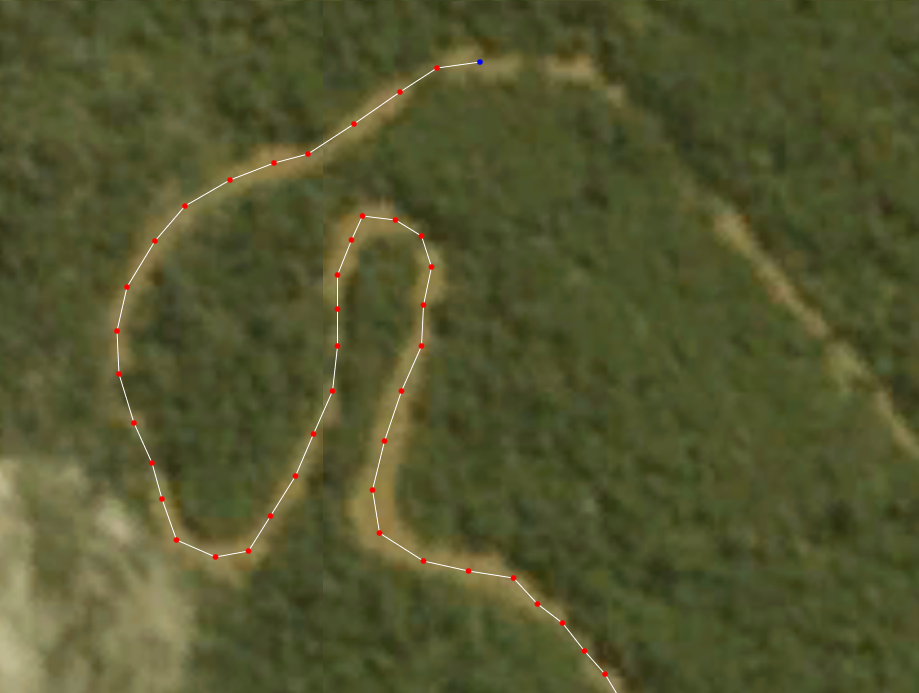
\includegraphics[width=0.957\linewidth]{GE_example_clickclick01_exc.png}
		\label{fig:goodlabel}
	\end{subfigure} 
	\begin{subfigure}{0.48\textwidth}
		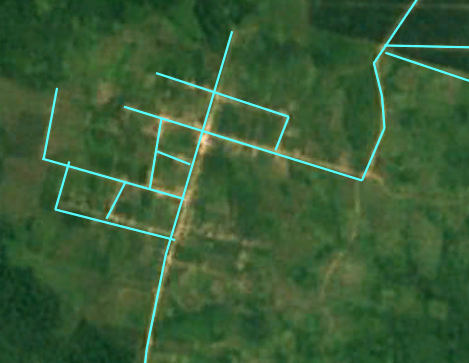
\includegraphics[width=0.957\linewidth]{GE_exemplaryScene_Borneo_allRoads_exc.png}
		\label{fig:badlabel}
	\end{subfigure} 
	\caption{Labeling roads. Left, example of an appropriate level of precision. The image is a screenshot of Google Earth while a small road was in the process of being labeled. Right, example of unacceptable labels. The labels are generally too imprecise; in particular, they are i) partially off-road, ii) incomplete (there are some gaps where roads join each other, and a whole winding road segment is missing in the bottom right quarter), iii) overshooting in some places. Likely, this is a result of labeling at a too zoomed-out level.}
	\label{fig:label_examples}
\end{figure}

Finally, we will start with the real work. \\

Be sure to have marked the layer created in the steps above, because all changes made to it will apply to the marked layer (Marking is done by clicking on the layer in the layer window).
Then, just to make sure the right tools are displayed, click on \textit{View} - \textit{Toolbars} - see if the Checkbox \textit{Digitizing Toolbar} is marked, if not, do so now. \\

Then, with the new labeling layer enabled and marked, click on the yellow pen symbol in the toolbar (which is situated on top of the QGIS window). \\
Now the layer editing mode is activated.
Near to the pen symbol, click on the line symbol marked with a little star (a tooltip should pop up if you hover over the icon stating something like: "Add Line Feature").  
When you now move the cursor to the map section of the screen, the cursor should change to a crosshair. \\

Now you can start clicking (diligently) along the roads, each point marking a new node of the line.
You can change to the hand tool during digitizing to move the map, or you can move across the map with the arrow keys. The middle mouse button will also do the job. \\

When done with a road, you can exit digitzing mode with a right click.
A window will pop up asking you for the ID (or any other attributes you specified).
The best practice would be to insert a running number per road, nothing too overcomplicated. 

\subsection{Saving the data}

When you are done, right click on the layer you created. \\
Click  \textit{export} - \textit{Save layer as} - and then choose either \textit{ESRI Shape File} or \textit{Keyhole Markup Language (KML)}.

Done. These files are the labels we need to do proper road detection.




%\section{A Short Introduction To Preprocessing: \newline Pixel Classification}

% Now after the introduction its time spread some info on how to actually do the thing :)  

%\subsection{Classification Preview}

%\subsection{Do A Classification}

% a classification can not do the labelling for you but is meant to help you decide in cases where roads are not easily visible








\end{document}
